The notch in the angular intensity of light reflected in the specular
direction arises due to interference between the specularly reflected beam
and the re-radiated SPP field anti-phase at the excitation angle,
$\thetasp$.  As most of the incident light is specularly reflected into
this direction, the notch is the most obvious spatial signature of surface
plasmon resonance in a prism-coupled configuration.  Much less obvious, but
equally important for the present discussion, is an additional optical
feature observable in the same half-space.

As first shown in SPOM experiments with near field probes, during propagation
roughness or other surface inhomogeneities can elastically modify the
in-plane momentum of an SPP\@.  This phenomena is known as ``directional
scattering'', the signature of which is a annular ``cone'' of light at
$\thetasp$ along an azimuthal coordinate $\phi$ (\Figure{fig:conefig}).
Though light in the cone is far less intense than in the specular
direction, it can be readily observed with the naked eye with a visible
laser of only a few milliwatts (e.g.\ a \SI{5}{\milli\watt} HeNe at
\SI{632.8}{\nano\meter}~\cite{schumann2009surface}).
\begin{figure}[ht]
 \centering
 \import{includes/}{setpgfinc}
 %\import{existence/figures/}{conefig}
 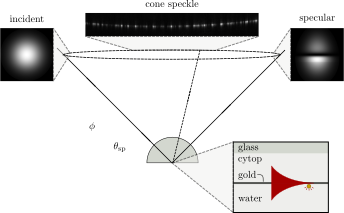
\includegraphics{existence/figures/conefig}
 \caption{Coordinates of the conically scattered light.}
\label{fig:conefig}
\end{figure}

The physical process responsible for directionally scattered light begins
with the transmission of the incident light at $\thetasp$ through the layer
structure, evanescently exciting SPPs.  This first transmission is
identified by the Fresnel \textit{forward} transmission coefficient,
$t^p_+$ (e.g.\ for a three-layer system with layers 0, 1, and 2, $t^p_+
\equiv t^p_{012}$).  Upon SPP re-radiation as a photon, light will take the
transmitted path in reverse, back through the layer structure into the
prism, which is identified by the Fresnel \textit{reverse} transmission,
$t^p_-$ (e.g.\  $t^p_- \equiv t^p_{210}$).  The intensity in the cone
$I_\mathrm{cone}$ is proportional to the product $t^p_+$ and $t^p_-$~\cite{simon1976directional},
\begin{equation}
I_\mathrm{cone}
= \frac{1}{I_0}\frac{\mathrm{d}I}{\mathrm{d}\Omega}
= 4 {\left(\frac{\omega}{c}\right)}^4 |t^p_+|^2
|t^p_-|^2\,W(\theta_i,\theta_s,\phi)\, |s(\Delta \mathbf{k})|^2
\label{eqn:guhacone},
\end{equation}
where $I_0$ is the incident optical power and
$\mathrm{d}I/\mathrm{d}\Omega$ is the scattered power per solid angle.
$s(\Delta \mathbf{k})$ is the surface roughness spectrum given by the Fourier
transform of the surface autocorrelation function,
\begin{equation}
|s(\Delta \mathbf{k})|^2 = \frac{\sigma^2}{4\pi} \left<S^2\right>
\me^{-(\Delta k^2 \sigma^2)/4}.
\label{eqn:surfaceroughness}
\end{equation}
The final term, $W(\theta_i,\theta_s,\phi)$, is a dipole function describing
the interference of two roughness-induced currents on the
surface~\cite{raether1997surface}.

For practical purposes, $W(\theta_i,\theta_s,\phi)$ and $s(\Delta
\mathbf{k})$ can be treated as constants if the incident Gaussian beam is
within a small angular range~\cite{heitmann1977determination}.  The angular
width of the cone is approximately
\begin{equation}
\theta_{1/2} = 2 k^{\prime\prime} \frac{c}{\omega \cos \theta},
\end{equation}
on the order of \SI{0.2}{\degree} for LRSPPs and \SI{4}{\degree} for
conventional SPs.  In this regard, $W(\theta_i,\theta_s,\phi)$ and
$s(\Delta \mathbf{k})$ will be neglected
except in a limited scope in \Chapter{ch:scatteringmicro}, such that
\begin{equation}
|E_\mathrm{cone}|^2 \propto	|t^p_+|^2 |t^p_-|^2.
\label{eqn:conefield}
\end{equation}

Due to the \textit{double} plasmonic enhancement in
\Equation{eqn:guhacone}, light in the cone has a smaller angular width than
its specular counterpart in the notch, shown in \Figure{fig:conevsnotch}
for a three-layer system ($n_1=1.5142$, $n_2=\num{0.2843 + 3.3825i}$,
$n_3=1.331$ and $d_2=\SI{45}{\nano\meter}$).  In \Figure{fig:conevsnotch},
the cone signal has been inverted and normalized to the same range as the
notch to facilitate this comparison.
%The smaller angular width will enhance
%This aspect causes certain measurements in
%the cone to be more sensitive than those in the notch, an aspect we will
%visit in \Section{sec:bulkri}.
\begin{figure}[ht]
\centering
\import{includes/}{setpgfinc}
\import{existence/figures/}{cone_vs_notch}
\caption{Comparison of the angular optical profile of the cone and notch.  The
cone signal has been inverted and normalized to the same range as the notch for
comparison.}
\label{fig:conevsnotch}
\end{figure}

The notch is the prime spatial feature of SPR biosensing in prism-coupled
setups and, as a result of the significant academic and commercial interest
in the field, it is very well understood.  Furthermore, advancements in the
engineering and implementation of such devices already achieved shot-noise
limited performance~\cite{piliarik2009surface}.  In contrast, very little
information is avaliable about the cone apart from a few material-science
oriented papers showing the utility of its integrated intensity in SPOM
measurements~\cite{kim1995scanning}, connection with surface
roughness~\cite{simon1976directional}, and angular polarization
distribution~\cite{kim1997conical}.  The present work attempts to addresses
this difficiency in the context of biosensing with new investigations into
the influence of the spatial intensity distribution in the cone on both
changes in bulk refractive index (\Section{sec:bulkri}) as well as
perturbations in the underlying scattering microstructure
(\Chapter{ch:scatteringmicro}).  In particular, it will be shown that under
certain conditions the cone contains optical speckle, which can be used
to great utility to sense discrete binding events which perturb the
scattering microstructure.
